\clearpage\null\vfill
\thispagestyle{empty}
\begin{minipage}[b]{.9\textwidth}
  \begin{center}
  \setlength{\parskip}{.5\baselineskip}
  {\color{phdcol0}%
   \ccLogo\hspace{.1cm}%
   \ccAttribution\hspace{.1cm}%
   \ccNonCommercial\hspace{.1cm}%
   \ccNoDerivatives}\hspace{.15cm}%
  \footnotesize%
  This work is licensed under {\color{phdcol1}\textbf{http://creativecommons.org/licenses/by-nc-nd/3.0/}}
  \end{center}
\end{minipage}
\vspace*{2\baselineskip}
\clearpage
\thispagestyle{empty}
\vspace*{\stretch{1}}
\begin{flushright}
  \textit{À Seref, Keziban, Didem et Ilayda.}
\end{flushright}
\vspace*{\stretch{7}}
%

\chapter*{Remerciements}

Je souhaite en premier lieu remercier mes encadrants Fabrice Kordon, 
Soheib Barrir et Maximilien Colange qui m'ont accompagné durant ma thèse.
Les discussions que nous avons eu m'ont permis d'avancer dans mes travaux de recherches.

Merci aux deux rapporteurs de ce travail, 
Laure Petrucci et Pascal Fontaine qui ont accepté de relire et évaluer ce manuscrit et également à 
tous les autres membres de mon jury Jean-Michel Couvreur, Emmanuelle Encrenaz et Bart Bogoerts.


Merci A Yann Thierry-Mieg pour toutes les discussions a propos des solveurs SAT et SMT et 
Julien Sopena  qui m'a fait découvrir le SAT durant mon stage de Master 1.


Je souhaite également remercier tous mes collègues des équipes Move, Delys et Whisper du LIP6 avec qui j'ai
pu partager 



Damien Carver
Gauthier Voron

Merci à mes co-bureau, Ludovic Le Frioux, Vincent Vallade 

Ilays Toumililt
Redha Gouicem
Maxime Bittan

Saalik Hatia

Rémi Oudin
Marjorie Bournat
Denis Jeanneau

Jonathan Sid-Otmane

Lucas Serrano
Antoine Blin

Francis Laniel
Florent Coriat
Arnaud Favier











%
%\`A tous, \textbf{merci infiniment} !
%

\chapter*{Résumé Long}


Cette thèse traite la résolution du problème de satisfaisabilité booléenne (SAT).
SAT permet de résoudre des problèmes importants dans différents domaines tels 
que la planification~\cite{planning_92}, la biologie~\cite{biology_06}, la vérification de logiciel et de 
matériel~\cite{biere1999symbolic}, de raisonnement automatique~\cite{heule2016solving}, etc.
Leurs évolutions au cours des dernières décennies leur ont permis de traiter des problèmes de plus en plus complexes.
Des travaux récents ont réussi a prouver à l'aide d'un solveur SAT, une borne maximum
pour le problème de coloration des triplets pythagoriciens, avec une preuve de 200 TB~\cite{heule2016solving}.


Étant donné un problème SAT, l'objectif est de  déterminer si il est possible de satisfaire toutes les contraintes du
problème, si c'est le cas on dit que le problème est satisfaisable, sinon il est insatifaisable.
% satisfaisable ou non.
%
% c'est à dire que toutes les contraintes peuvent être satisfaites,
%ou insatisfaisable, c'est-à-dire qu'il n'y a aucun moyen de satisfaire toutes les contraintes avec une même affectation.
Ce calcul est effectué par un solveur SAT qui répond $\sat$ lorsque la formule est satisfaisable et $\unsat$ dans le cas
contraire. SAT a été le premier problème ayant été prouvé NP-Complet~\cite{cook1971complexity}. Cela signifie que
l'on ne connait pas d'algorithme capable de résoudre le problème avec une complexité polynomiale.
%La résolution du problème est l'un des sept prix du millénaire, à savoir P = NP.


Malgré cette complexité, les solveurs SAT sont capables de résoudre de plus en plus de problèmes complexes.
Ce succès vient de l'introduction de différentes heuristiques sophistiquées dans 
l'algorithme de résolution le plus répandu, $\guillemotleft$ Conflict Driven Clause Learning$\guillemotright$ (CDCL).
Il est basé sur l'algorithme DPLL nommé suivant ses auteurs Davis, Putnam, Logemann et Loveland~\cite{dpll_62},
et est l'un des premiers algorithmes avec une utilisation non intensive de la mémoire.

%
%Cet algorithme est basé sur  
%et Loveland (DPLL)\cite{dpll_62}.
%
%
%l'optimisation de l'algorithme de
%résolution des conflits appelé $\guillemotleft$ Conflict Driven Clause Learning$\guillemotright$ (CDCL) qui est basée sur le premier
%algorithme (avec une utilisation non intensive de la  mémoire) nommé par ses auteurs Davis, Putnam, Logemann
%et Loveland (DPLL)\cite{dpll_62}.

%Le CDCL peut être vu suivant l'exploration d'un arbre binaire avec au total $2^n$ branches, avec $n$ le nombre de variables du problème.
%La première étape consiste à choisir une variable dite de décision, puis d'effectuer les déductions logiques à partir de l'affection. 
%Si l'algorithme se trouve dans une situation de conflit, c'est-à-dire que 
%
% que l'affectation courante n'est pas capable de satisfaire au moins une contrainte du problème, l'algorithme  calcule une clause dite de conflit qui permet d'élaguer 
%cet espace de recherche. Avec cette contrainte le solveur effectue un \textit{backjump}, c'est-à-dire qu'il remonte dans l'arbre
%de recherche pour explorer une autre branche.
%%Cette clause est une information redondante par rapport au problème initial.
%Si aucun conflit n'est présent, l'algorithme choisit à nouveau une variable de décision. L'algorithme termine  soit lorsque toutes les variables sont affectées auquel cas le problème est satisfaisable, soit lorsque un conflit est apparu avec uniquement des déductions logiques auquel cas le
%problème est non satisfaisable.
%La Figure~\ref{fig:cdclflow} présente sous forme d'un organigramme le fonctionnement de l'algorithme CDCL.
%
\begin{figure}[!htbp]
\begin{tikzpicture}[node distance=1.5cm,
,every node/.style={scale=0.7,fill=white, font=\sffamily}, align=center]
% Specification of nodes (position, etc.)
\tikzset{%	
	>={Latex[width=2mm,length=2mm]},
	% Specifications for style of nodes:
	base/.style = {rectangle, rounded corners, draw=black,
		minimum width=2cm, minimum height=1cm,
		text centered, font=\sffamily},
	question/.style = {base, diamond, fill=blue!15},
	unsat/.style = {base, fill=red!30,minimum width=3cm},
	sat/.style = {base, fill=green!30,minimum width=3cm},
	process/.style = {base, minimum width=2.5cm, fill=orange!15,
		font=\ttfamily},
}
\node (isfin) [question] {Variables toutes \\assignées ?};
\node (dec)     [process, below = of isfin]          {Choix variable \\ de decision};
\node (sdec)     [right = of dec]          {};
\node (idec) [left = of isfin]  {};
\node (prop)    [process, below = of dec ]          {Propagation unitaire};
\node (conf)    [question, below = of prop] { Conflit ?};
\node (confanalyse) [process, below = of conf] {Analyse du \\ conflit};
\node (learn) [process] at ($(prop) + (160pt, 0)$) {Apprentissage de la \\ clause de conflit};
\node (isend) [question] at ($(confanalyse) + (160pt, 0)$) {Niveau de \\decision zero ?};
\node (end) [unsat] at ($(isend) + (140pt, 0)$) {$\unsat$};
\node (ends) [sat] at ($(isfin) + (+160pt, 0)$){$\sat$};


\draw[->, thick]     (sdec) -- (dec);
\draw[->, thick]     (dec) -- (prop);
\draw[->, thick]     (prop) -- (conf);
\draw[->, thick]     (conf) -| node [yshift=5.5 cm] {non}(idec.center) -- (isfin);
\draw[->, thick]     (conf) -- node {oui} (confanalyse);
\draw[->, thick]     (isfin) -- node {non}(dec);
\draw[->, thick]     (confanalyse) --(isend);
\draw[->, thick]     (isend) -- node {oui}(end);
\draw[->, thick]     (isfin) -- node {oui}(ends);
\draw[->, thick]     (learn) -- (prop);
\draw[->, thick]     (isend) -- node [] {non}(learn);

\end{tikzpicture}
\caption{Organigramme de l'algorithme CDCL}
\label{fig:cdclflow}
\end{figure}

%\begin{figure}[!htbp]
%	\begin{tikzpicture}[node distance=1.5cm,
%	,every node/.style={scale=0.7,fill=white, font=\sffamily}, align=center]
%	% Specification of nodes (position, etc.)
%	\tikzset{%	
%		>={Latex[width=2mm,length=2mm]},
%		% Specifications for style of nodes:
%		base/.style = {rectangle, rounded corners, draw=black,
%			minimum width=2cm, minimum height=1cm,
%			text centered, font=\sffamily},
%		question/.style = {base, diamond, fill=blue!15},
%		unsat/.style = {base, fill=red!30,minimum width=3cm},
%		sat/.style = {base, fill=green!30,minimum width=3cm},
%		process/.style = {base, minimum width=2.5cm, fill=orange!15,
%			font=\ttfamily},
%	}
%	\node (isfin) [question] {All vars\\ assign?};
%	\node (dec)     [process, below = of isfin]          {Choose decision var};
%	\node (sdec)     [right = of dec]          {};
%	\node (idec) [left = of isfin]  {};
%	\node (prop)    [process, below = of dec ]          {Unit Propagation};
%	\node (conf)    [question, below = of prop] { IsConflict?};
%	\node (confanalyse) [process, below = of conf] {Conflict Analysis};
%	\node (learn) [process] at ($(prop) + (160pt, 0)$) {Learn conflict clause};
%	\node (isend) [question] at ($(confanalyse) + (160pt, 0)$) {is level\\zero?};
%	\node (end) [unsat] at ($(isend) + (140pt, 0)$) {$\unsat$};
%	\node (ends) [sat] at ($(isfin) + (+160pt, 0)$){$\sat$};
%	
%	
%	\draw[->, thick]     (sdec) -- (dec);
%	\draw[->, thick]     (dec) -- (prop);
%	\draw[->, thick]     (prop) -- (conf);
%	\draw[->, thick]     (conf) -| node [yshift=5.5 cm] {no}(idec.center) -- (isfin);
%	\draw[->, thick]     (conf) -- node {yes} (confanalyse);
%	\draw[->, thick]     (isfin) -- node {no}(dec);
%	\draw[->, thick]     (confanalyse) --(isend);
%	\draw[->, thick]     (isend) -- node {yes}(end);
%	\draw[->, thick]     (isfin) -- node {yes}(ends);
%	\draw[->, thick]     (learn) -- (prop);
%	\draw[->, thick]     (isend) -- node [] {no}(learn);
%	
%	\end{tikzpicture}
%	\caption{Organigramme de l'algorithme CDCL}
%	\label{fig:cdclflow}
%\end{figure}



%Parmi eux, certains problèmes présentent des symétries et créent une
%explosion combinatoire qui entrave les performances du solveur. Celui-ci explore en vain
%les parties identiques (isomorphes) de l’espace de recherche. 
%



Même si les solveurs sont de plus en plus efficace, certains problèmes ne peuvent pas être résolus.
Parmi eux, certains problèmes présentent des symétries, dans ce cas, des branches de l'espace de recherche 
sont identiques à une permutation près, on dit que cet espace de recherche est isomorphe.
Si une branche de l'espace de recherche est solution du problème alors toutes les branches symétriques
sont également des solutions. Dans le cas inverse si il n'existe pas de solution dans une branche alors il n'en
existe dans aucune des branches symétriques.
En parcourant les espaces isomorphes, le solveur effectue donc du travail inutile.

Pour illustrer ce problème, prenons comme exemple le problème des tiroirs (\textit{pigeonhole problem}) dans lequel nous avons un ensemble de pigeons qui doivent êtres attribués à des nids différents. Dans ce problème il y a un nid de moins que le nombre de pigeons.
Le but de ce problème est de déterminer s'il est possible d'attribuer un nid différent à chaque pigeon.
La figure~\ref{fig:holefr} présente une instance de ce problème.

\begin{figure}[!htbp]
	\centering
	\begin{tikzpicture}[
	start chain = going right,
	node distance = 0pt,
	AStyle/.style={draw, minimum width=2em, minimum height=2em, 
		outer sep=0pt, on chain, fill=yellow!0!white}]
	\node [AStyle] (1) {\huge\textcolor{gray}{\PHdove}};
	\node [AStyle] (4) {\huge\textcolor{gray}{\PHdove}};
	\node [AStyle] (5) {\huge\textcolor{gray}{\PHdove}};
	\node [AStyle, draw] (6) {\huge\textcolor{gray}{\PHdove}};
	\node [ minimum width=2em, minimum height=2em, 
	outer sep=1pt, on chain] (7) {\huge\textcolor{gray}{\PHdove}};
	\end{tikzpicture}
	\caption{Représentation graphique d'une instance du problème des pigeons (5 pigeons, 4 nids)}
	\label{fig:holefr}
\end{figure}


Pour un humain, la réponse à ce problème est évidente, mais un solveur de l'état de l'art va parcourir toutes 
les combinaisons possibles de couples (pigeon, nid) et cela le mène à une explosion combinatoire.
Pour cette raison, résoudre ce problème avec un solveur SAT standard s'avère très chronophage et même impossible 
dans des temps raisonnables pour un nombre de pigeons supérieur à 15.

%Cependant, certains problèmes possèdent un espace de recherche énorme et ne peuvent pas 
%être traité par un solveur SAT. Un exemple d'un tel problème peut être le problème de tournées de véhicules (VRP). 
%Il s'agit du service d'entreprise de livraison, dans lequel étant donné une flotte de véhicules basés dans un dépôt, ceux ci doivent faire des rondes entre des clients qui ont demandés chacun une certaine quantité de marchandises. Le circuit effectué par un véhicule pour la visite de tous les clients
%est appelé la tournée du véhicule. L'objectif est de trouver la tournée qui minimise les coûts de livraison (monétaire, distance, temps, ....).
%
%
%Dans le problème précédent, renommer l'ensemble de véhicules identiques nous donnera exactement le même problème. C'est ce qu'on appelle une symétrie.

De manière plus  générale, une symétrie est une transformation qui laisse un objet (ou un aspect de l'objet) inchangé. Les symétries sont généralement définies comme une propriété syntaxique d'un problème lorsque leur présence est inhérente à l'encodage du problème.
Dans ce cas, une permutation des variables préserve la spécification originale du problème.
Dans le cas où les symétries sont indépendantes d'une représentation particulière du problème, il s'agit de symétries sémantiques.


La présence de symétrie dans un problème force l'algorithme de recherche à explorer en vain l'espace de recherche symétrique et impacte considérablement ses performances.  La rupture de symétrie est une approche qui évite au solveur de visiter les espaces de recherche isomorphes.

Pour pouvoir exploiter les symétries, la première étape consiste à les trouver. Dans le contexte de la satisfaction booléenne, la détection des symétries syntaxiques se fait tout d'abord par la transformation de la spécification en un graphe coloré et ensuite par l'application d'un outil d'automorphisme de graphe sur celui-ci.
Différents outils traitent de ce problème dans l'état de l'art, tels que, $\bliss$~\cite{JunttilaKaski:ALENEX2007}, $\saucy$~\cite{katebi2010symmetry}, …


Lorsque les symétries sont obtenues, la façon la plus courante pour les exploiter est d'utiliser une approche de rupture de symétrie statique. Elle est dite statique, car le traitement de cette approche  est effectuée avant la résolution du problème SAT.
Ceci consiste à prendre le problème symétrique en entrée et à produire une formule à satisfaction équivalente, en éliminant les symétries présentes. %Le problème en sortie ne peut pas être insatisfaisable si le problème initial est satisfaisable.
Pour produire une formule équivalente sans présence de symétries, le problème est augmenté par des 
contraintes de rupture de  symétries  (\textit{symmetry breaking predicates sbp)}.
 Celles-ci empêchent le solveur d'explorer les espaces de recherche isomorphes. 
Si l'on considère l'exemple précédent avec les pigeons, le premier pigeon est attribué a un
exactement un nid, la symétrie est alors «rompue».

Plusieurs outils, tels que $\shatter$~\cite{aloul06} et $\breakid$~\cite{devriendt2016improved}, utilisent cette technique pour accélérer le calcul du solveur en présence de symétries.
En général, cette approche aboutit à de bons résultats dans différentes instances symétriques, cependant elle possède des défauts. Parmi eux, nous pouvons citer le nombre de contraintes ajoutées qui peut être exponentiel par rapport à la taille du problème. Ceci a pour conséquence de ralentir l'algorithme principal du solveur au lieu de l'accélérer.
De plus, étant donné que ce calcul est effectué avant le lancement du solveur, cette approche peut être difficilement combinée avec d'autres techniques de rupture de symétries. Aussi, cette approche ne peut pas distinguer les contraintes originales du problème avec les contraintes de rupture de symétrie. Avec cette information, le solveur peut modifier ses heuristiques pour augmenter ses performances. Pour ces raisons, certains problèmes avec de nombreuses symétries ne peuvent pas être traités efficacement avec cette approche.

Une autre approche dite rupture de symétrie dynamique consiste à utiliser les symétries durant l'algorithme de recherche du solveur SAT, plus précisément, à modifier son comportement pour exploiter les propriétés de symétrie du problème. Cette approche consiste à déduire des faits symétriques par rapport aux déductions effectuées par le solveur. Lorsque ces faits sont ignorés, le solveur explore en vain l'espace de recherche symétrique.
Ces déductions réduisent le nombre de décisions, qui sont des suppositions du solveur choisies de 
manière heuristique, et augmentent le nombre de propagations qui sont les déductions logiques faites par le solveur. 
Cette approche transforme donc les suppositions du solveur en déductions logiques et accélère donc le solveur.
Différents outils utilisent cette approche, nous pouvons citer \textit{Symmchaff}~\cite{sabharwal2005symchaff}
qui n'exploite que certains types spécifiques de symétries, \textit{Symmetry Propagation (SP)}~\cite{Devriendt12}, \textit{Symmetry Learning Scheme (SLS)}~\cite{benhamou2010enhancing} et \textit{Symmetry Explanation Learning (SEL)}~\cite{devriendt2017symmetric} qui ajoutent les symétriques des clauses apprises pour permettre les déductions symétriques.
Étant donné que cette approche est dynamique, il est possible pour le solveur 
d'intégrer des heuristiques spécifiques ou encore de combiner les différentes techniques de rupture de symétrie.
Cependant cette approche n'est pas efficace sur certaines instances qui sont très facilement résolues avec l'approche statique
et vice-versa.


Cette thèse vise à améliorer l'existant et rendre les solveurs plus performants en présence de symétries et
propose différentes contributions allant dans ce sens.  



Notre première contribution mime le comportement de la rupture de symétrie statique, mais 
opère dynamiquement, pendant l'exécution du solveur. On ajoute dans le solveur un composant de symétrie
qui va détecter que le solveur parcourt un espace de recherche symétrique et va ajouter à celui-ci de une contrainte appelée $\guillemotleft$ effectective symmetry breaking predicate $\guillemotright$ qui va empêcher le solveur de rester dans
l'espace de recherche en question. 



% Cette contrainte est dite effective, car 
% à l'inverse de l'approche 
%de rupture de symétrie  statique la contrainte est forcément utilisée par le solveur. Aucune contrainte
%inutile n’est insérée dans le solveur. 

Ce composant de symétrie est fourni sous forme d'une bibliothèque codée en C++ et se nomme $\libdsb$.
Elle peut s'interfacer avec n'importe quelle solveur de type CDCL avec très peu de ligne de code. 
Pour conduire nos expériences, nous l'avons interfacée avec un solveur de l'état de l'art nommé $\minisat$~\cite{een2003extensible}. Au total, l'intégration de $\libdsb$ ajoute environ 60 lignes de code 
et augmente le code de $\minisat$ de 3\%.
$\libdsb$ est $\guillemotleft$ open source $\guillemotright$, fourni sous une licence GPLv3 et est disponible sur Github \footnote{\url{https://github.com/lip6/cosy}}.


Pour évaluer notre approche, nous avons comparé une version du solveur $\minisat$ combiné avec la bibliothèque $\libdsb$, que nous avons appelé $\cdclsym$ avec les solveurs de l'état de l'art.
Ces expérimentations ont été effectuées sur les instances de la SAT Competiton~\cite{jarvisalo2012international} sur les dernières années (2012 - 2017) pour lesquelles $\bliss$ a réussi a trouver des symétries. Au total, nous avons obtenu 1350 instances.

La figure~\ref{fig:frcactus} nous montre les résultats obtenus sous forme d'un cactus plot, 
dans lequel l'axe des abscisses nous montre le nombre d'instances réussies par chacun des solveurs et l'axe des ordonnées nous montre le temps de calcul des solveurs.
Nous avons conduit ces expériences avec deux outils d'automorphisme de graphe, à savoir 
$\saucy$ à gauche de la figure et $\bliss$ à droite de la figure. 

Comme nous pouvons le constater, les résultats sont meilleurs  avec l'utilisation de l'outil d'automorphisme de 
graphe $\bliss$. La principale différence entre les deux outils est le nombre de permutations obtenues.
$\bliss$ nous donne plus de permutations que $\saucy$, cela permet a notre outil $\cdclsym$ d'atteindre 
un nombre d'instances résolues de 775 alors que le deuxième meilleur outil $\breakid$ atteint un nombre d'instances résolues de 749 avec $\bliss$. Toutes les expériences étaient limitées à une durée à 5000 secondes.

Ces expériences nous démontrent que notre approche est aussi performante que les approches de rupture de symétrie statique.
\begin{figure}[!htbp]
	\centering
	\subfloat[avec \saucy]{{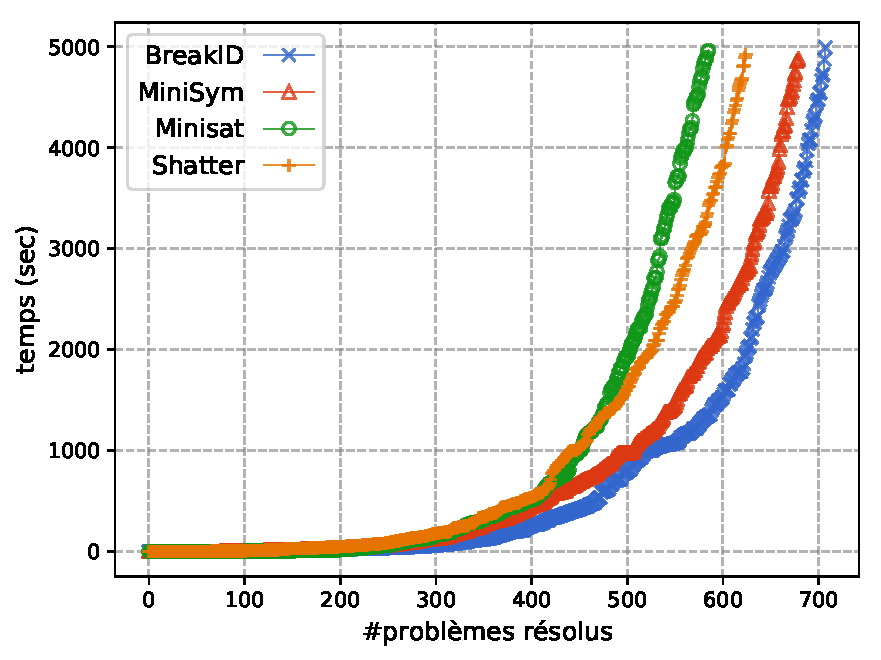
\includegraphics[scale=0.36]{img/saucy-fr}}}%
	\qquad
	\subfloat[with \bliss]{{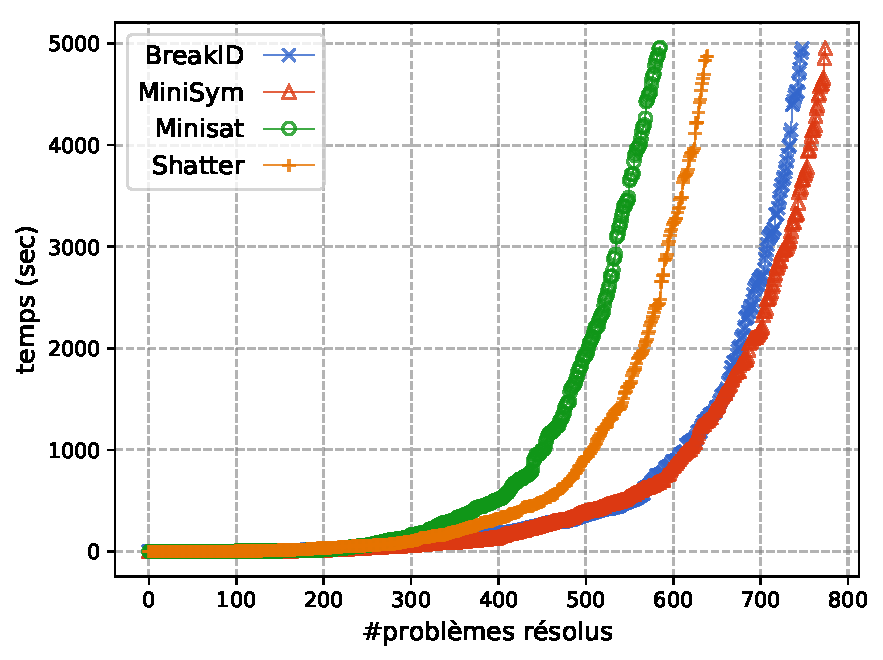
\includegraphics[scale=0.36]{img/bliss-fr}}}%
	\caption{Cactus plot  présentant le nombre total d'intances résolues}%
	\label{fig:frcactus}%
\end{figure}

Malgré les très bons résultats obtenus par notre approche, certains problèmes qui sont résolus très 
rapidement par les approches de rupture de symétrie dynamique tel que  Symmetry Propagation (SP) ne pouvaient toujours pas être traité par notre approche et vise-versa.
SP est une approche qui a pour but d'accélérer la traversée de l'espace de recherche en déduisant des faits symétriques à partir des déductions effectuées par le solveur.
À l'inverse notre approche consiste à éliminer les espaces de recherche 
symétriques. %Ces deux approches sont donc orthogonales.
Notre deuxième contribution consiste à déterminer si cette combinaison est possible. Elle se résume donc à la question suivante:
Est-il possible d'accélérer la traversée de l'espace de recherche tout en éliminant les espaces de symétriques ?

Pour que cette approche soit correcte, la contrainte qu'il faut absolument respecter est que la symétrie utilisée pour déduire les faits symétriques doit être valide dans le problème. En effet, les clauses ajoutées pour éliminer l'espace de recherche
symétrique vont rompre cette symétrie. Cette dernière ne peut donc plus être utilisée pour propager les faits symétriques.
Une approche naïve est de supprimer chacune des symétries dès lors qu'une contrainte de rupture de symétrie a été ajoutée.
Le problème avec cette approche est que l'ensemble vide est très vite atteint et donc que plus aucune déduction symétrique ne peux être faite. Notre approche consiste à traquer les clauses utilisées par le solveur et à connaître à tout instant l'ensemble des symétries valide. Au lieu de considérer les symétries au niveau de la formule,
notre approche consiste a utiliser les symétries au niveau de la clause (locale).


\vspace{2em}


\begin{table}[!htbp]\footnotesize
	\centering
	\resizebox{.65 \textwidth}{!}{
	\begin{tabular}{lcccc}
		Solver & PAR-2 & TOTAL & SAT & UNSAT\\
		\toprule
		\texttt{Minisat SP} & 1674h00 & 876 & 406 & 470 \\
		\texttt{Minisat Sym} & 1578h30 & 904 & 416 & 488\\
		\texttt{Minisat SymSP} & \cellcolor{gray!30}\textbf{1570h15} & \cellcolor{gray!30}\textbf{911} & \cellcolor{gray!30}\textbf{420} & \cellcolor{gray!30}\textbf{491}\\	
	\end{tabular}
	
	}
	\caption{Comparaison du nombre de problèmes résolus par chaque approche.}
	\label{tab:satfr}
\end{table}%


%\begin{table}[!htbp]\footnotesize
%	\centering
%	\resizebox{1 \textwidth}{!}{
%		\begin{tabular}{l|ccc}
%			\toprule
%			Benchmark  &\texttt{minisat-Sp} & \texttt{minisat-Sym} & \texttt{minisat-SymSP}\\
%			\hline 
%			Permutations 0–20 (704) & \cellcolor{gray!30,}\textbf{233}&220&226\\
%			Permutations 20–40 (136) & 50&\cellcolor{gray!30}\textbf{54}&\cellcolor{gray!30}\textbf{54}\\
%			Permutations 40–60 (141) & 75&\cellcolor{gray!30}\textbf{83}&\cellcolor{gray!30}\textbf{83}\\
%			Permutations 60–80 (168) & \cellcolor{gray!30}\textbf{11}&\cellcolor{gray!30}\textbf{11}&10\\
%			Permutations 80–100 (51) & \cellcolor{gray!30}\textbf{11}&\cellcolor{gray!30}\textbf{11}&\cellcolor{gray!30}\textbf{11}\\
%			Permutations \textgreater100 (200) & 90&\cellcolor{gray!30,}\textbf{109}&107\\
%			\hline 
%			TOTAL no dup (1400) & 470&488&\cellcolor{gray!30,}\textbf{491}\\
%			\bottomrule
%		\end{tabular}
%	}
%	\caption{Comparaison des approches sur les instances UNSAT.}
%	\label{tab:unsatfr}
%\end{table}

Les expérimentations pour évaluer les performances de l'approche se sont effectuées sur les instances de la SAT Competiton sur sept années (2012 - 2018) pour lesquelles $\bliss$ a trouver des symétries. Au total, nous avons obtenu un total de 1400 instances.Les trois solveurs comparés sont respectivement \texttt{Minisat SP}, le solveur $\minisat$ avec l'approche SP; \texttt{Minisat Sym} le solveur $\minisat$ avec $\libdsb$ et \texttt{Minisat-SymSP} le solveur avec l'approche combiné.
La table \ref{tab:satfr} présentent les résultats obtenues pour les problèmes SAT et UNSAT.
Les différent solveurs sont comparés selon quatre mesures, PAR-2 qui représente le temps cumulé de chaque solveur 
avec une pénalité pour les instances non résolues, \-TOTAL qui représente le nombre total d'instances résolues, SAT le nombre d'instances satisfaisable résolues et UNSAT le nombre d'instances  non satisfaisable résolues.
Globalement, nous observons que l'approche combinée améliore les résultats avec un gain d'environ 8 heures par rapport
à \texttt{Minisat Sym} et de 104 heures par rapport à \texttt{Minisat SP}. Le nombre total d'instances résolues est également
supérieur aux autres solveurs.



%Cette deuxième contribution réponds à la question, Est-il possible d'accélérer la traversée de l'espace de recherche tout en éliminant l'espace de symétrique ?
%La réponse est positive grâce à l'introduction des symétries locales. 


\chapter*{Résumé}

Le problème de satisfaisabilité booléenne consiste à trouver une solution à une formule  propositionnelle.
Ce problème NP-complet peut modéliser une grande variété de problèmes industriels et académiques couvrant la planification, la résolution des dépendances, la vérification formelle, l'optimisation logique, la cryptographie, etc.
Les  progrès récents ont permis de mettre au point des solveurs SAT très efficaces, capables de traiter des millions de variables et des millions de contraintes. 
Les compétitions internationales SAT mettant en vedette des modèles industriels mettent au défi et stimulent le développement de solveurs SAT de plus en plus efficaces.


Dans la pratique, de nombreux systèmes présentent des symétries ce qui permet de raisonner sur une abstraction quotient de l'espace de recherche, basée sur des classes d'équivalence par rapport aux symétries, et réduire exponentiellement l'espace de recherche dans les cas favorables.
Dans cette thèse, nous explorons comment exploiter les réductions de symétrie pour améliorer les performances des solveurs SAT.


Les approches existantes pour exploiter les symétries dans la résolution SAT, consistent à calculer les symétries du problème puis à générer des "prédicats de rupture de symétrie statique" qui s'ajoutent au problème, obligeant le solveur à adopter un seul représentant pour chaque classe d'équivalence des solutions.
Le problème avec cette approche est que le nombre de contraintes supplémentaires peut être plus important que le problème original et peut surcharger le solveur. La première contribution de cette thèse appelée CDCL[sym] est un nouvel algorithme léger et dynamique, qui n'introduit ces contraintes supplémentaires de rupture de symétrie que de manière opportuniste au fur et à mesure que le solveur progresse.

Une deuxième approche pour exploiter les symétries consiste en ce qu'on appelle la rupture de symétrie dynamique qui s'intéresse à la propagation symétrique des \textit{deductions} du solveur lorsque cela est possible.
Cette approche résout certains modèles que la rupture de symétrie statique ne peut résoudre, et vice-versa, mais à notre connaissance, ces approches n'avaient jamais été combinées avec succès. 
Dans notre deuxième contribution de cette thèse, nous combinons cette stratégie avec la précédente. permettant pour la première fois la propagation à la volée de déductions symétriques tout en continuant à bénéficier des avantages de CDCL[sym].

Tous les algorithmes présentés dans cette thèse ont été mis en implémentés et largement testés à l'aide de grands benchmarks issus de compétitions SAT. Le solveur SAT sensible à la symétrie développé au cours de cette thèse s'avère compétitif par rapport à l'état de l'art et, dans de nombreux cas symétriques, est capable de surpasser les autres solveurs.

%Aujourd'hui, la satisfaction booléenne (SAT) est un domaine de recherche actif qui trouve son application dans différents domaines tels que l'optimisation logique, la génération de motifs de test, la vérification formelle et la simulation fonctionnelle, etc.
%Par conséquent, l'élaboration d'approches qui pourraient traiter des problèmes SAT 
%de plus en plus complexes est devenue une priorité.
%Certains problèmes présentent des symétries et créent une explosion combinatoire qui entrave les performances du solveur. Celui-ci explore en vain les parties symétriques de l'espace de recherche.
%
%Dans l'état de l'art, il existe deux approches qui traitent de ce problème, la première, appelée \textit{rupture de symétrie statique}, vise à enrichir le problème d'origine avec des contraintes qui empêchent le solveur d'explorer
%les espaces de recherches symétriques. Le second appelé \textit{rupture de symétrie dynamique} ajoute une composante de symétrie dans le noyau du solveur et modifier son comportement pour l'accélérer le parcours de l'espace de recherche en utilisant les symétries présentes dans le problème initial. Ces approches sont efficaces mais n'arrivent néanmoins pas à traiter l'ensemble des instances symétriques.
%
%
%Dans cette thèse, nous avons cherché à mieux exploiter les propriétés de symétrie des problèmes.
%Pour ce faire, nous proposons deux contributions majeures qui visent à améliorer les approches de l'état de l'art et à augmenter le nombre d'instances résolues. La première imite le comportement de l'approche de \textit{rupture de symmétrie statique} mais fonctionne dynamiquement. Un contrôleur de symétrie au sein du solveur observe son comportement  et génère des contraintes de rupture de symétries de manière opportuniste.
%La seconde vise à combiner l'approche précédente avec une approche dynamique. Le but est de prendre le meilleur de deux mondes,
%accélérer le parcours du solveur en utilisant des symétries tout en l'empêchant de visiter les parties symétriques de l'espace de recherche.
%
%Des expériences approfondies sur le benchmark des compétitions SAT montrent que nos approches sont compétitives et même meilleures dans certains cas avec les meilleures approches de l'état de l'art.


\chapter*{Abstract}

%
%Nowadays, logic is omnipresent and it is used in different domains such as 
%One method to solve this kind of problem is satisfiability problem (SAT).
%SAT solvers are more and more powerful and can handle large problems which seemed to be infeasible 
%few years ago. However, some problems present symmetries which force the solver to explore fruitlessly
%the symmetric part of the search space and hinders the performance. 


% SAT important : NP-complete, solver efficaces depuis 2000+, problèmes de taille croissante (indus), 
% benchmarks + compétitions reconnues
Boolean satisfiability (SAT) solves the problem of finding a solution to a propositional Boolean formula.
This NP-complete problem can model a wide variety of industrial and academic problems
covering planning, dependency resolution, formal verification, logic optimization, cryptography\ldots
Recent advances have led to very efficient SAT solvers, able to deal with millions of variables and 
constraints. International SAT competitions featuring industrial models challenge and drive the
 development of ever more efficient SAT solvers.
 
% symmetry important
Many systems in practice exhibit symmetries, that can allow to reason on a quotient abstraction of the 
search space, based on equivalence classes with respect to the symmetries, that can be exponentially smaller than the full search space in favorable cases.
In this thesis, we explore how to exploit symmetry reductions to improve the performance of SAT solvers.

% SOTA 1 : static
Existing approaches to exploit symmetries in SAT solving, consist in computing the symmetries of the problem 
then generating so-called "static symmetry breaking predicates" that are added to the problem, forcing the solver to 
adopt only one representative for each equivalence class of solutions.
% limite + contrib
% contribution 1 : CDCL-sym online symmetry breaking
The problem with this approach is that the number of additional constraints can be larger than the original system,
 and may overload the solver. The first contribution of this thesis called CDCL[sym] is a novel lightweight and dynamic algorithm,  that only introduces these additional symmetry breaking constraints opportunistically as the solver progresses.
 
% SOTA 2 : dynamic
A second approach to exploit symmetries consists in so-called \textit{dynamic symmetry breaking} that
is concerned with symmetric propagation of the \textit{deductions} of the solver when possible.
This approach solves some models that static symmetry breaking cannot solve, and vice-versa,
but to our knowledge these approaches had never been successfully combined. 
In our second contribution of this thesis, we combine this strategy with the previous
approach,  enabling for the first time on the fly propagation of symmetric deductions 
 while still gaining the benefits of CDCL[sym].

All the algorithms presented in this thesis have been implemented and extensively tested using large benchmarks taken from SAT competitions. The symmetry aware SAT solver developed during this thesis is shown to be competitive with the state of the art
and in many symmetric cases is able to outperform all other solvers.



%adds a symmetry component to the solver core
%and modifies its behavior to accelerate it using symmetries presents in the initial problem.
%These approaches are effective but are not able to handle all symmetric instances.
%% contrib 2 : symmetry propagation + breaking
%The second one aims to combine the previous approach with a dynamic one. The goal is to take best of both worlds,
%accelerate the solver's tree traversal  by using symmetries while preventing him from visiting the symmetrical parts of the research space.
%
%
%
%In the state-of-the-art two majors approaches that address  this problem, the first, called \textit{static symmetry breaking}
%aims to enrich the original problem problem with constraints that prevents the solver from exploring
%symmetric parts of the search space. 
%
%In this thesis, we set out to exploit symmetry properties of the problems in better ways.
%For this purpose, we propose two major contributions that aims to improve the state-of-the-art approaches and augment the number of solved symmetric instances.
%% contrib 2 : symmetry propagation + breaking
%The second one aims to combine the previous approach with a dynamic one. The goal is to take best of both worlds,
%accelerate the solver's tree traversal  by using symmetries while preventing him from visiting the symmetrical parts of the research space.
%% contrib 3 : tool + mesures + experiments
%Extensive experiments on the benchmark of SAT competitions show that our approaches are competitive and even better 
%in some cases with the best state-of-the-art approaches.
